\begin{frame}
	\frametitle{``Fake'' Lepton Background}
	
	\vspace{15pt}
	\li{QCD jet production ($\rightarrow$ ``fake'' leptons) ill described by MC $\rightarrow$ use the Matrix Method.}
		\lii{Exploits the different
probabilities for ``real'' and ``fake'' leptons to
pass from ``loose'' to ``tight'' cuts}
		\lii{Using {\color{orange}measurable} quantities to calculate {\color{purple}truth} quantities}
			
		\vspace{-5pt}
		%\begin{center}\makebox[.7\textwidth][c]{%
		\begin{minipage}{.5\linewidth}
			\begin{equation*}
			\psBox{orange!30}{
  		  		\begin{pmatrix} 
				N_{T} \\
				N_{L} 
				\end{pmatrix}
				}=
				\begin{pmatrix}
				\epsilon_{R} & \epsilon_{F} \\
				1 - \epsilon_{R} & 1 - \epsilon_{F}
				\end{pmatrix}
				\psBox{purple!30}{
				\begin{pmatrix}
				N_{R} \\
				N_{F}
				\end{pmatrix}
				}
 		 	\end{equation*} 
		\end{minipage}\hfill
		\begin{minipage}{.4\linewidth}
			\begin{equation*}
			\boxed{
 				\epsilon_{F} = \frac{N^{fake}_{tight}}{N^{fake}_{loose}}, \, \,  
 				\epsilon_{R} = \frac{N^{real}_{tight}}{N^{real}_{loose}}
 				}
  			\end{equation*}
		\end{minipage}
		\vspace{10pt}
		\cleft{.25}
		\vspace{10pt}
		\li{From the first line:}
		\cright{.75}
		\begin{equation*}
  	\begingroup
  		\color{ATLASBlue_lighter}\overbrace{\color{black}				\highlight[ATLASBlue_lighter]{N_{T}}}^{\mathclap{\text{\color{ATLASBlue}signal selection}}}
  %\highlight[ATLASBlue_lighter]{N_{T}} 
  \endgroup
  \,\,= \,\,
  \begingroup
  \color{highgreen}\underbrace{\color{black}\highlight[highgreen]{\epsilon_{R}N_{R}}}_{\mathclap{\text{\color{green}contribution from real electrons}}}
  %\highlight[highgreen]{\epsilon_{R}N_{R}} 
  \endgroup
  \,\,+ \,\,
  \begingroup
  \color{highred}\overbrace{\color{black}\highlight[highred]{\epsilon_{F}N_{F}}}^{\mathclap{\text{\color{red}contribution from fake electrons}}}
  %\highlight[highred]{\epsilon_{F}N_{F}}
  \endgroup \,\,\, \, ,
\end{equation*}
\cend

\li{Inverting matrix yields ``fake'' component in data (tight selection):}
\vspace{10pt}
		\begin{equation*}
			\epsilon_{F}N_{F} = \frac{\epsilon_{F}}{\epsilon_{R} - \epsilon_{F}} \big[ \epsilon_{R}(N_{L} + N_{T}) - N_{T} \big]	
		\end{equation*}
		
		\vspace{-10pt}
\end{frame}
	

\begin{frame}
	\frametitle{``Fake'' Lepton Background}
	\vspace{10pt}
	\li{Loose Selection:}
		\lii{{\bfseries $e$:} signal selection except LHTight ID \& isolation $\rightarrow$ only LHMedium / LHLoose. }
		\lii{{\bfseries $\mu$:} signal selection except isolation}			
	\li{Tight Selection: same as signal selection.}

	\vspace{20pt}
		\begin{minipage}{0.44\textwidth}
			\begin{center}
				{\bfseries REAL}
			\end{center}
		\end{minipage}
		\begin{minipage}{0.52\textwidth}
			\begin{center}
				{\bfseries FAKE}
			\end{center}
		\end{minipage}\par\medskip
		\begin{minipage}{0.44\textwidth}
			\begin{itemize}
				\item Count real $\ell$ candidates passing selections.
				\item Estimate $\epsilon_{R}$ with W MC and truth matching ($\Delta$R < 0.2).
				\item \pt\, and $\eta$ dependency $\rightarrow$ 2D binning.
			\end{itemize}
		\end{minipage}
		\begin{minipage}{0.52\textwidth}
			\begin{itemize}
				\item Calculate using data.
				\item Cut to suppress genuine $\ell$\, from W \& Z.
				\item Account for contamination with real $\ell$\, with MC {\footnotesize (subtract real-electron dilution from fake rate)}.
				\item Binned in \pt\, and $\abs{\Delta\phi_{e,\met} }$.
			\end{itemize}
		\end{minipage}
	
\end{frame}		


\begin{frame}
	\frametitle{Fake Rates}
	
	\cleft{.5}
	\begin{center}
		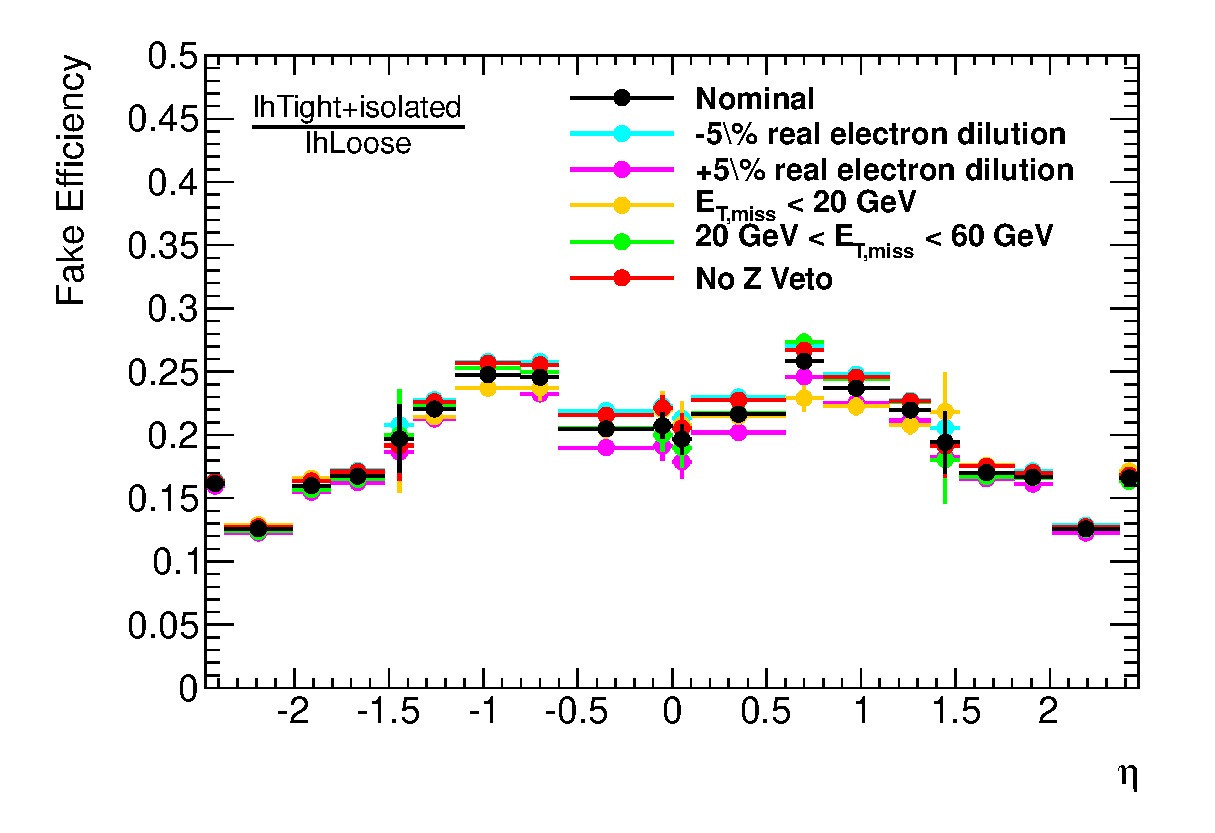
\includegraphics[width=.7\linewidth]{plots/RealsFakesMine/TL_FakeRate_eta_F.eps}\\
		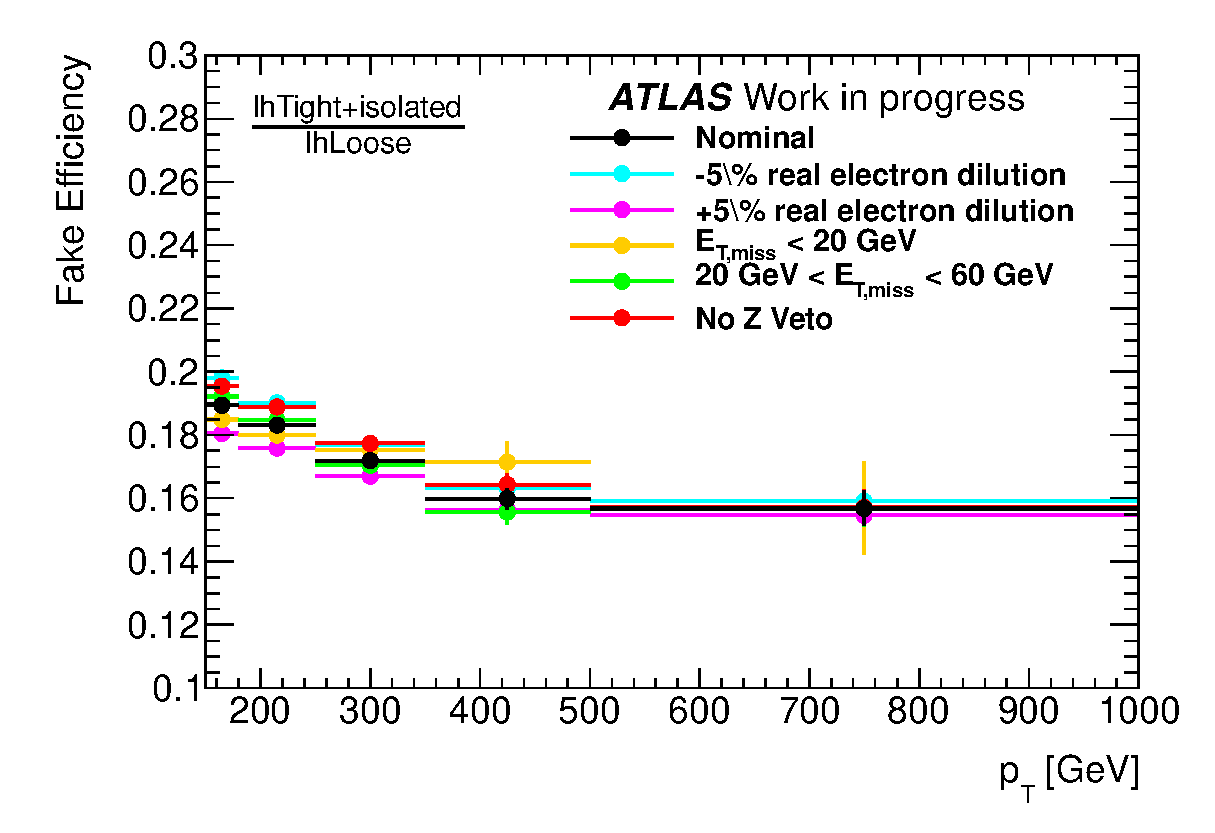
\includegraphics[width=.7\linewidth]{plots/RealsFakesMine/TL_FakeRate_pt_F.eps}
	\end{center}
	\cright{.5}
	\begin{center}
		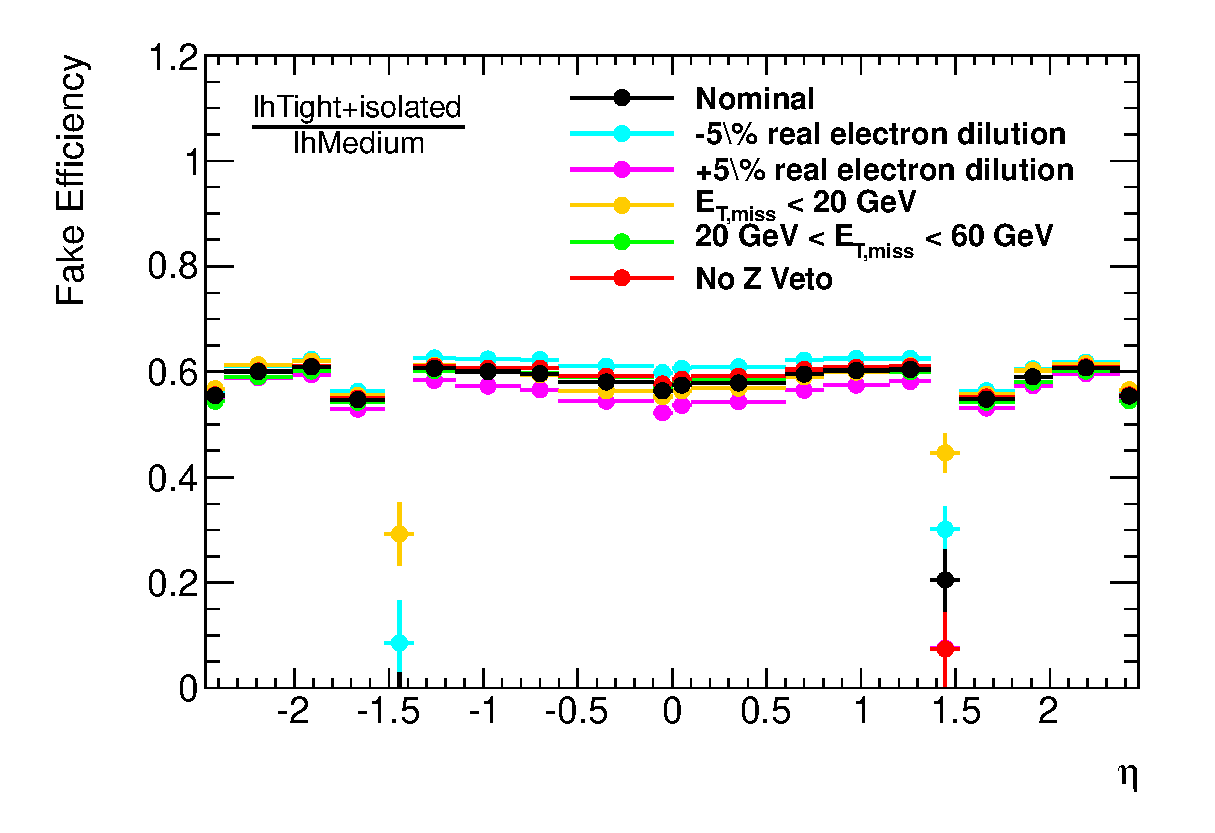
\includegraphics[width=.7\linewidth]{plots/RealsFakesMine/TM_FakeRate_eta_F.eps}\\
		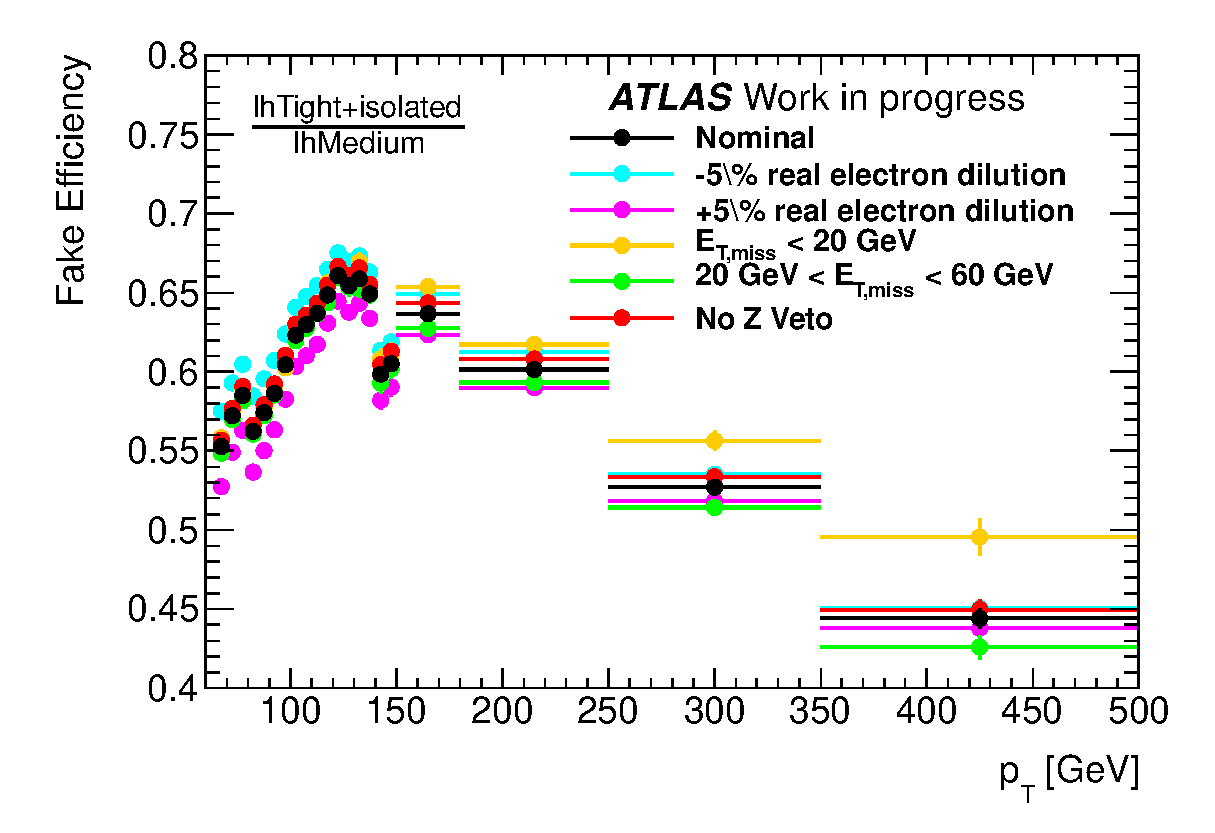
\includegraphics[width=.7\linewidth]{plots/RealsFakesMine/TM_FakeRate_pt_F.eps}
	\end{center}
	\cend
\end{frame}

\begin{frame}
	\frametitle{Real Rates}
	
	\cleft{.25}
	\cright{.5}
	\begin{center}
		\includegraphics[width=.7\linewidth]{plots/RealsFakesMine/ALL_RealRate_eta_F.eps}
	\end{center}
	\cright{.25}
	\cend
	\vspace{-10pt}
	\cleft{.5}
	\begin{center}
		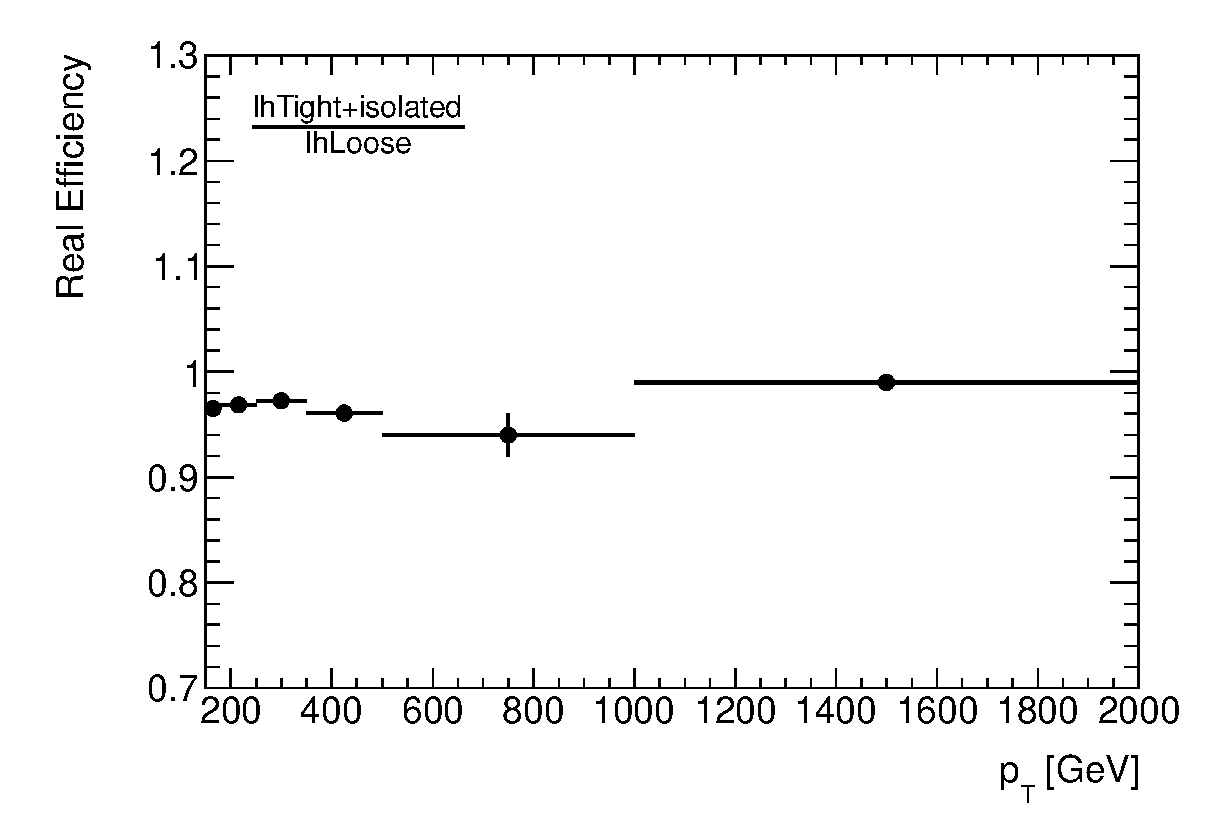
\includegraphics[width=.7\linewidth]{plots/RealsFakesMine/TL_RealRate_pt_F.eps}
	\end{center}
	\cright{.5}
	\begin{center}
		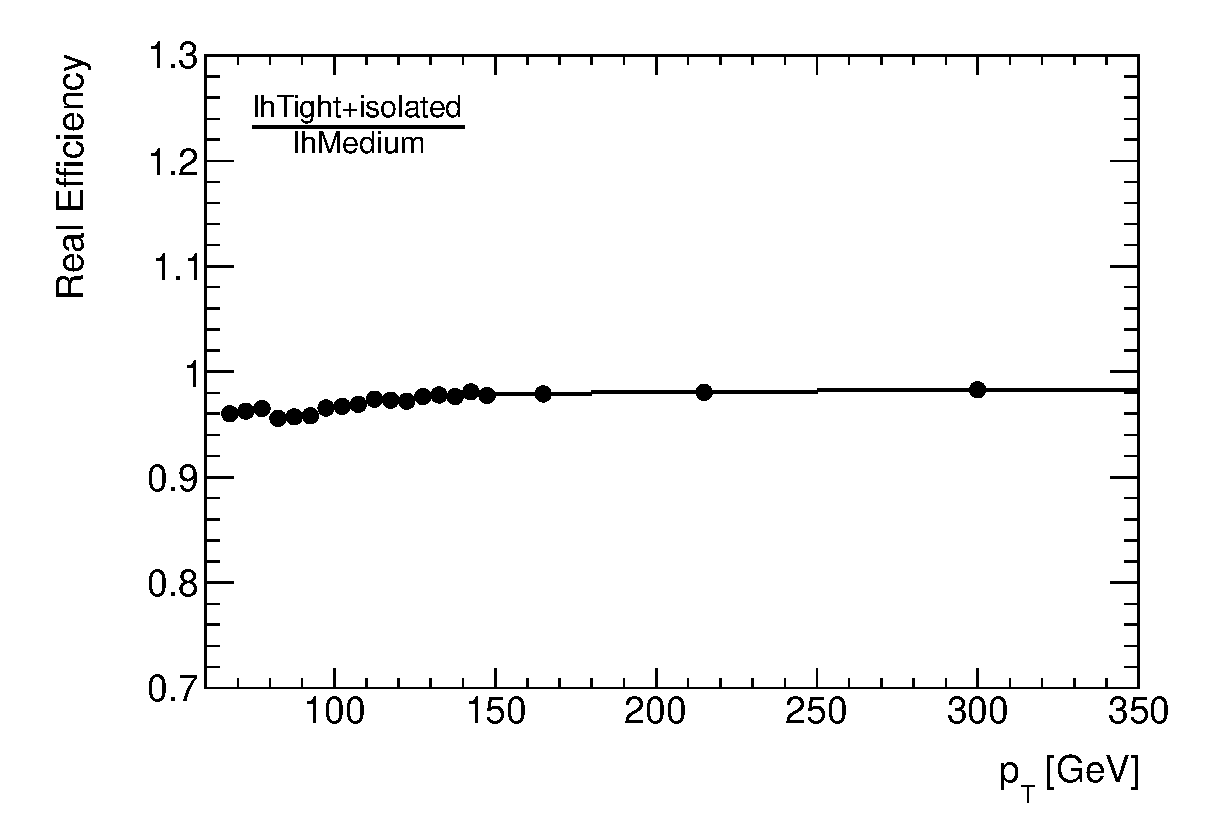
\includegraphics[width=.7\linewidth]{plots/RealsFakesMine/TM_RealRate_pt_F.eps}
	\end{center}
	\cend
\end{frame}